\documentclass[a4paper, 12pt, final, garamond]{book}
\usepackage{cours-preambule}

\raggedbottom

\makeatletter
\renewcommand{\@chapapp}{M\'ecanique -- chapitre}
\makeatother

\begin{document}
\setcounter{chapter}{2}

\chapter{Correction TD entra\^inement}
\section{Glissade d'un pingouin sur un igloo}
\begin{enumerate}
    \item 
        \begin{itemize}[label=$\diamond$, leftmargin=10pt]
            \litem{Système~:} \{pingouin\}
        \end{itemize}
        \begin{minipage}{0.70\linewidth}
            \begin{itemize}[label=$\diamond$, leftmargin=10pt]
                \litem{Référentiel~:} $\Rc\ind{sol}$ supposé galiléen
                \litem{Repère~:} $(\Or, \ur, \ut)$ avec $\ut$ \textbf{dans le sens de
                    $\tt$}
                \litem{Repérage~:}
                \vspace*{-12pt}
                    \begin{align*}
                        \OM(t) &= R\ur\\
                        \vf(t) &= R\tp\ut\\
                        \af(t) &= R\tpp\ut - R\tp^2\ur
                    \end{align*}
            \end{itemize}
        \end{minipage}
        \hfill
        \begin{minipage}{0.25\linewidth}
            \begin{center}
                \hspace*{-3cm}
                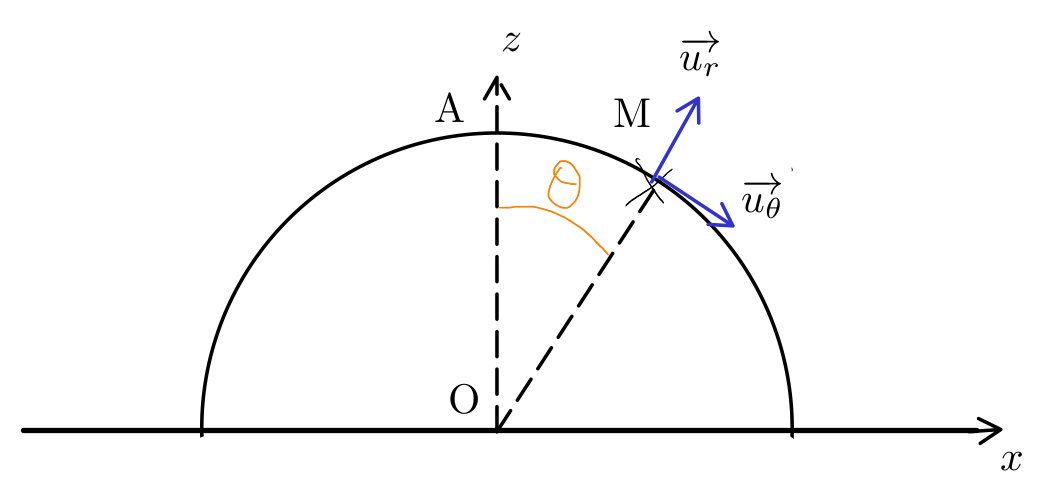
\includegraphics[width=1.8\linewidth]{igloo_corr}
            \end{center}
        \end{minipage}
        \vspace*{12pt}
        \begin{itemize}[label=$\diamond$, leftmargin=10pt]
            \litem{Origine et instant initial~:}
            \begin{gather*}
                \OM(0) = \vv{\rm OA} \Ra \tt(0) = 0\\
                \vf(0) = \of \Ra \tp(0) = 0
            \end{gather*}
            \litem{BDF~:}
                \[
                    \begin{array}{ll}
                        \textbf{Poids} & \Pf = mg(-\cos\tt\ur +\sin\tt\ut)\\
                        \textbf{Réaction} & \Rf = R_N\ur
                    \end{array}
                \]
            \item \leftcenters{\textbf{PFD~:}}{
                    $\DS
                    m\af = \Pf + \Rf
                    \Lra
                    \mqty(-mR\tp^2\\mR\tpp) = \mqty(-mg\cos\tt+R_N\\mg\sin\tt)
                    $}
                    \begin{empheq}[box=\fbox, left=\Lra\empheqlbrace]{align}
                        \label{eq:pinga}
                        R_N  & = mg\cos\tt - mR\tp^2\\
                        \label{eq:pingb}
                        \tpp & = \frac{g}{R}\sin\tt
                    \end{empheq}
        \end{itemize}
        L'équation du mouvement est celle qui donne l'équation d'oscillateur
        harmonique aux petits angles, et qu'on a déjà utilisée en cours sur le
        pendule, et linéaire en $\tt$~: l'équation~\eqref{eq:pingb}.
        L'équation~\eqref{eq:pinga} contient l'information sur le contact à
        l'igloo.
    \item En prenant~\eqref{eq:pingb}$\times\tp$, on a
        \begin{align*}
            \tpp\tp
                &= \frac{g}{R} \tp\sin\tt
            \\\Lra
            \dv{t}(\frac{1}{2}\tp^2)
                &= \frac{g}{R} \dv{t}(-\cos\tt)
            \\\Lra
            \frac{1}{2}\int_{t=0}^{t} \dv{\tp^2}{t}\dt
                &= \frac{g}{R}\int_{t=0}^{t} \dv{(-\cos\tt)}{t}\dt
            \\\Lra
            \frac{1}{2} \left[ \tp^2 \right]_{t=0}^{t}
                &= \frac{g}{R} \left[ -\cos\tt \right]_{t=0}^{t}
            \\\Lra
            \Aboxed{\tp^2 &= \frac{2g}{R}(1-\cos\tt)}
            \qed
        \end{align*}
    \item En reprenant~\eqref{eq:pinga}, on peut remplacer $\tp^2$~:
        \begin{align*}
            R_N &= mg\cos\tt -m\cancel{R}\frac{2g}{\cancel{R}}(1-\cos\tt)
            \\\Lra
            \Aboxed{R_N &= mg(3\cos\tt -2)}
        \end{align*}
    \item La condition de support d'un solide est $R_N > 0$~: le pingouin
        décolle du support si la force de réaction est nulle, soit $R_N = 0$.
        Or,
        \begin{align*}
            R_N &= 0
            \\\Lra
            3\cos\tt - 2 &=0
            \\\Lra
            \Aboxed{\tt &= \arccos(\frac{2}{3})}
        \end{align*}
        Une application numérique donne \fbox{$\tt = \ang{48.2}$}.
\end{enumerate}

\section{Course de F1}
\begin{enumerate}
    \item La voiture A d'\textsc{Alonso} entame son virage dès qu'elle passe par
        l'axe $\D$, et parcourt un demi-cercle de longueur
        \[\boxed{D_A = \pi R_A = \SI{283}{m}}\]
        En revanche, la voiture B de \textsc{Button} continue en ligne droite
        sur une distance $R_A-R_B$ avant d'entamer son virage, et parcourt de
        nouveau la même distance en ligne droite avant la sortie du virage.
        Ainsi,
        \[\boxed{D_B = 2(R_1-R_2) + \pi R_B = \SI{266}{m}}\]
        La voiture B parcourt moins de distance que la voiture A, mais
        \textbf{il est impossible d'en conclure quoi que ce soit} puisqu'on ne
        sait pas si les deux trajectoires sont parcourues à la même vitesse.
    \item Lorsqu'elles sont sur la partie circulaire de leur trajectoire,
        parcourue à vitesse constante (en norme), l'accélération (en norme) des
        voitures vaut
        \[a = \frac{v^2}{R} = \num{0.8}g\]
        puisque les pilotes prennent tous les risques. Ainsi,
        \[
            \boxed{v_A = \sqrt{aR_A} = \SI{26.6}{m.s^{-1}}}
            \qet
            \boxed{v_B = \sqrt{aR_B} = \SI{24.3}{m.s^{-1}}}
        \]
    \item Calculons le temps mis par chacun des pilotes pour passer le virage.
        On sait que
        \[\Dt = \frac{D}{v}\]
        d'où les résultats
        \[
            \boxed{\Dt_A = \SI{10.6}{s}}
            \qet
            \boxed{\Dt_B = \SI{10.9}{s}}
        \]
        Finalement, \textsc{Alonso} va plus vite que \textsc{Button} pour
        parcourir le virage~: \textbf{la meilleure trajectoire est la meilleure
        des deux}. À ne pas tenter en vérifiant chez soi, mais de quoi briller
        sur Mario Kart…?
\end{enumerate}

\section{Entraînement d'une spationaute}
\begin{itemize}[label=$\diamond$] %, leftmargin=10pt]
    \litem{Système~:} \{spationaute\}
    \litem{Référentiel~:} référentiel du laboratoire, supposé galiléen
    \litem{Repère~:} $(\Or,\ur,\ut)$ avec $\ut$ selon le sens de rotation
\end{itemize}
\begin{minipage}{0.60\linewidth}
    \begin{itemize}[label=$\diamond$] %, leftmargin=10pt]
        \litem{Repérage~:}
            \begin{align*}
                \vv{\rm OS}(t) &= L\ur\\
                \vf_S(t) &= L\w\ut\\
                \af_S(t) &= L\dot{\w}\ut -L\w^2\ur
            \end{align*}
    \end{itemize}
\end{minipage}
\hfill
\begin{minipage}{0.35\linewidth}
    \begin{center}
        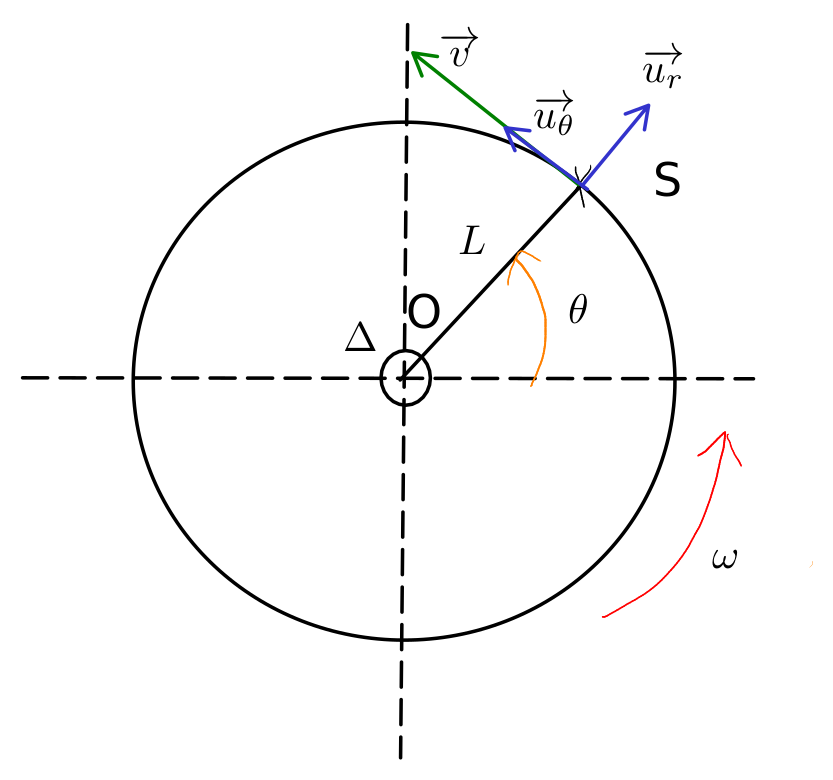
\includegraphics[scale=0.15]{spationaute_corr}
    \end{center}
\end{minipage}
\hfill
\begin{enumerate}
    \item Cf. schéma.
    \item Fait en introduction
    \item Au bout de quelques $\tau$, $\w(t) = \w_0$ et le mouvement sera
        circulaire uniforme. Les vecteurs vitesse et accélération deviennent~:
        \begin{empheq}[box=\fbox, left=\empheqlbrace]{align*}
            \vf_S(t) &= L\w_0\ut\\
            \af_S(t) &= -L\w_0{}^2\ur
        \end{empheq}
        La norme de l'accélération subie est alors \fbox{$\norm{\af_S} =
        L\w_0{}^2$}.
    \item ~
        \vspace{-24pt}
        \begin{gather}
            a_S = 10g \Ra \boxed{\w_0 = \sqrt{\frac{10g}{L}}}
            \qavec
            \left\{
                \begin{array}{rcl}
                    g & = & \SI{9.81}{m.s^{-2}}\\
                    L & = & \SI{10.0}{m}
                \end{array}
            \right.\\
            \AN
            \boxed{\w_0 = \SI{3.13}{rad.s^{-1}} \approx \SI{0.50}{tour.s^{-1}}}
        \end{gather}
\end{enumerate}

\begin{brema}{Ordres de grandeurs}
    \begin{itemize}[label=$\diamond$]
        \item Accélération latérale en F1~: \SIrange{4}{5}{g}~;
        \item Accélération latérale en avion de chasse~: \SIrange{9}{10}{g}
            pendant quelques secondes max~;
        \item Accélération verticale, éjection d'un avion de chasse~: $\approx
            \SI{20}{g}$ (interdiction de vol après 2 utilisation du siège
            éjectable à cause – notamment – du tassement des vertèbres)~;
        \item Accélération négative frontale en accident de voiture~:
            \SIrange{40}{60}{g}~! Même sans choc physique, une telle
            décélération cause des hémorragies internes à cause des organes
            internes percutant les os. Soyez prudent-es.
    \end{itemize}
\end{brema}

\section{Anneau sur une tige en rotation}
\begin{enumerate}
    \item
        \begin{minipage}[t]{0.60\linewidth}
            \begin{itemize}[label=$\diamond$, leftmargin=10pt]
                \litem{Système~:} \{anneau\} point matériel M de masse $m$
                \litem{Référentiel~:} terrestre supposé galiléen
                \litem{Repère~:} cylindrique $(\Or,\er,\et,\ez)$
                \litem{Repérage~:}
                    \begin{align*}
                        \OM &= r\er\\
                        \vf &= \rp\er + r\tp\et\\
                            &= \rp\er + r\w\et\\
                        \af &= \rpp\er + \rp\tp\et + \rp\w\et - r\w^2\er +
                            \underbracket[0.4pt]{\of}_{\dot{\w}=0}\\
                            &= (\rpp -r\w^2)\er +2r\w\et
                    \end{align*}
            \end{itemize}
        \end{minipage}
        \hfill
        \begin{minipage}[t]{0.35\linewidth}
            ~
            %\vspace*{6cm}
            \begin{center}
                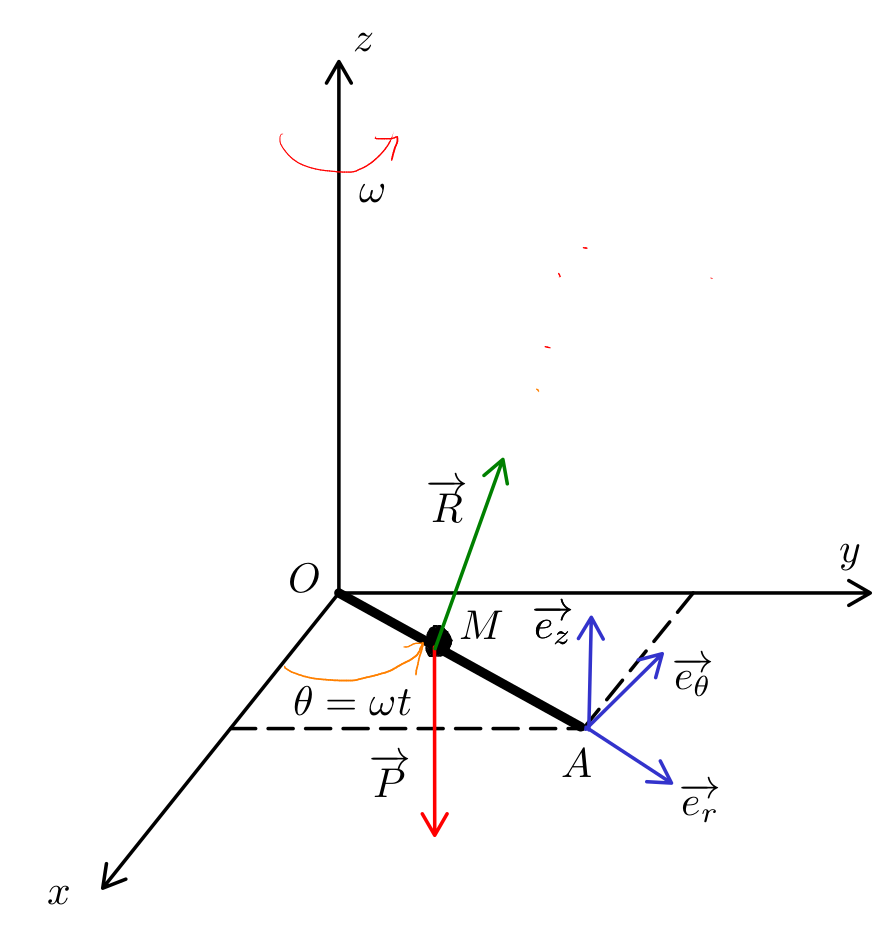
\includegraphics[scale=.18]{tige_rot_corr}
            \end{center}
        \end{minipage}
        \begin{itemize}[label=$\diamond$, leftmargin=10pt]
            \litem{Conditions initiales~:}
                \[
                    r(0) = r_0
                    \qet
                    \vf(0) = \of \Ra \rp(0) = 0
                \]
            \litem{BDF~:} pas de frottements donc pas de composante sur $\er$~:
                \[
                    \begin{array}{ll}
                        \textbf{Poids} & \Pf = m\gf = -mg\ez\\
                        \textbf{Réaction support} & \Rf = R_\tt\et + R_z\ez
                    \end{array}
                \]
            \litem{PFD~:}
                \begin{gather*}
                    m\af = \Pf + \Rf
                    \Lra
                    \left\{
                        \begin{aligned}
                            m(\rpp-r\w^2) & = 0\\
                            2m\rp\w       & = R_\tt\\
                            0             & = -mg + R_z
                        \end{aligned}
                    \right.
                \end{gather*}
                \begin{empheq}[box=\fbox, left=\Lra\empheqlbrace]{align}
                    \label{eq:tigerota}
                    \Aboxed{
                        \rpp - \w r &= 0
                    }\\
                    \label{eq:tigerotb}
                    R_\tt &= 2m\rp\w\\
                    \label{eq:tigerotc}
                    R_z &= mg
                \end{empheq}
        \end{itemize}
    \item On résout~\eqref{eq:tigerota} avec l'équation caractéristique~:
        \begin{align*}
            \rpp -\w^2r &= 0
            \\\Ra
            s^2 - \w^2 &= 0
            \\\Lra
            s^2 &= \w^2
            \\\Lra
            \Aboxed{s &= \pm\w}
        \end{align*}
        On a donc des solutions de la forme
        \begin{gather*}
            r(t) = A\exr^{\wt} + B\exr^{-\wt}
            \shortintertext{Or, avec les CI~:}
            \begin{aligned}
                r(0) &= r_0
                \\\Lra
                \Aboxed{r_0 &= A+B}
            \end{aligned}
            \shortintertext{et}
            \begin{aligned}
                \rp(0) &= 0
                \\\Lra
                0 &= A\w -B\w
                \\\Lra
                \Aboxed{A &= B}
            \end{aligned}
            \shortintertext{Soit}
            \\
            \boxed{A = B = \frac{r_0}{2}}
            \Ra
            \boxed{r(t) = \frac{r_0}{2}(\exr^{\wt} + \exr^{-\wt}) =
            r_0\cosh(\wt)}
        \end{gather*}
    \item On reprend~\eqref{eq:tigerotb} et~\eqref{eq:tigerotc} avec $\rp =
        \w r_0\sinh(\wt)$~:
        \[
            \boxed{
            \Rf = 2mr_0\w^2\sinh(\wt)\et + mg\ez
            }
        \]
    \item L'anneau quitte la tige en $\tau$ quand $r(\tau) = \ell$, soit
        \begin{gather*}
            \ell = r_0\cosh(\wt)
            \\\Lra
            \boxed{\tau = \frac{1}{\w}\acosh(\wt)}
        \end{gather*}
\end{enumerate}

\section{Pendule conique}
\begin{enumerate}
    \item On utilisera un repère cylindrique pour étudier la rotation.
    \item 
        \begin{itemize}[label=$\diamond$, leftmargin=10pt]
            \litem{Système~:} \{M\} masse $m$
            \litem{Référentiel~:} $\Rc\ind{labo}$ supposé galiléen
            \litem{Repère~:} $(\Or, \ur, \ut, \uz)$ (voir schéma)
        \end{itemize} \smallbreak
        \begin{minipage}{0.65\linewidth}
            \begin{itemize}[label=$\diamond$, leftmargin=10pt]
                \litem{Repérage~:} $R = \cte\Ra\dot{R} = 0$, $\tp = \w =
                    \cte\Ra\dot{\w} = 0$~:
                    \begin{align*}
                        \OM       & = R\ur = L\sin\a\ur\\
                        \vf_{\Mr} & = L\tp\sin\a\ut\\
                                  & = L\w\sin\a\ut\\
                        \af_{\Mr} & = -L\w^2\sin\a\ur
                    \end{align*}
                \litem{BDF~:}
                    \[
                        \begin{array}{ll}
                            \textbf{Poids} & \Pf = m\gf = -mg\uz\\
                            \textbf{Tension} & \Tf = T(-\sin\a\ur + \cos\a\uz)
                        \end{array}
                    \]
            \end{itemize}
        \end{minipage}
        \hfill
        \begin{minipage}{0.30\linewidth}
            \begin{center}
                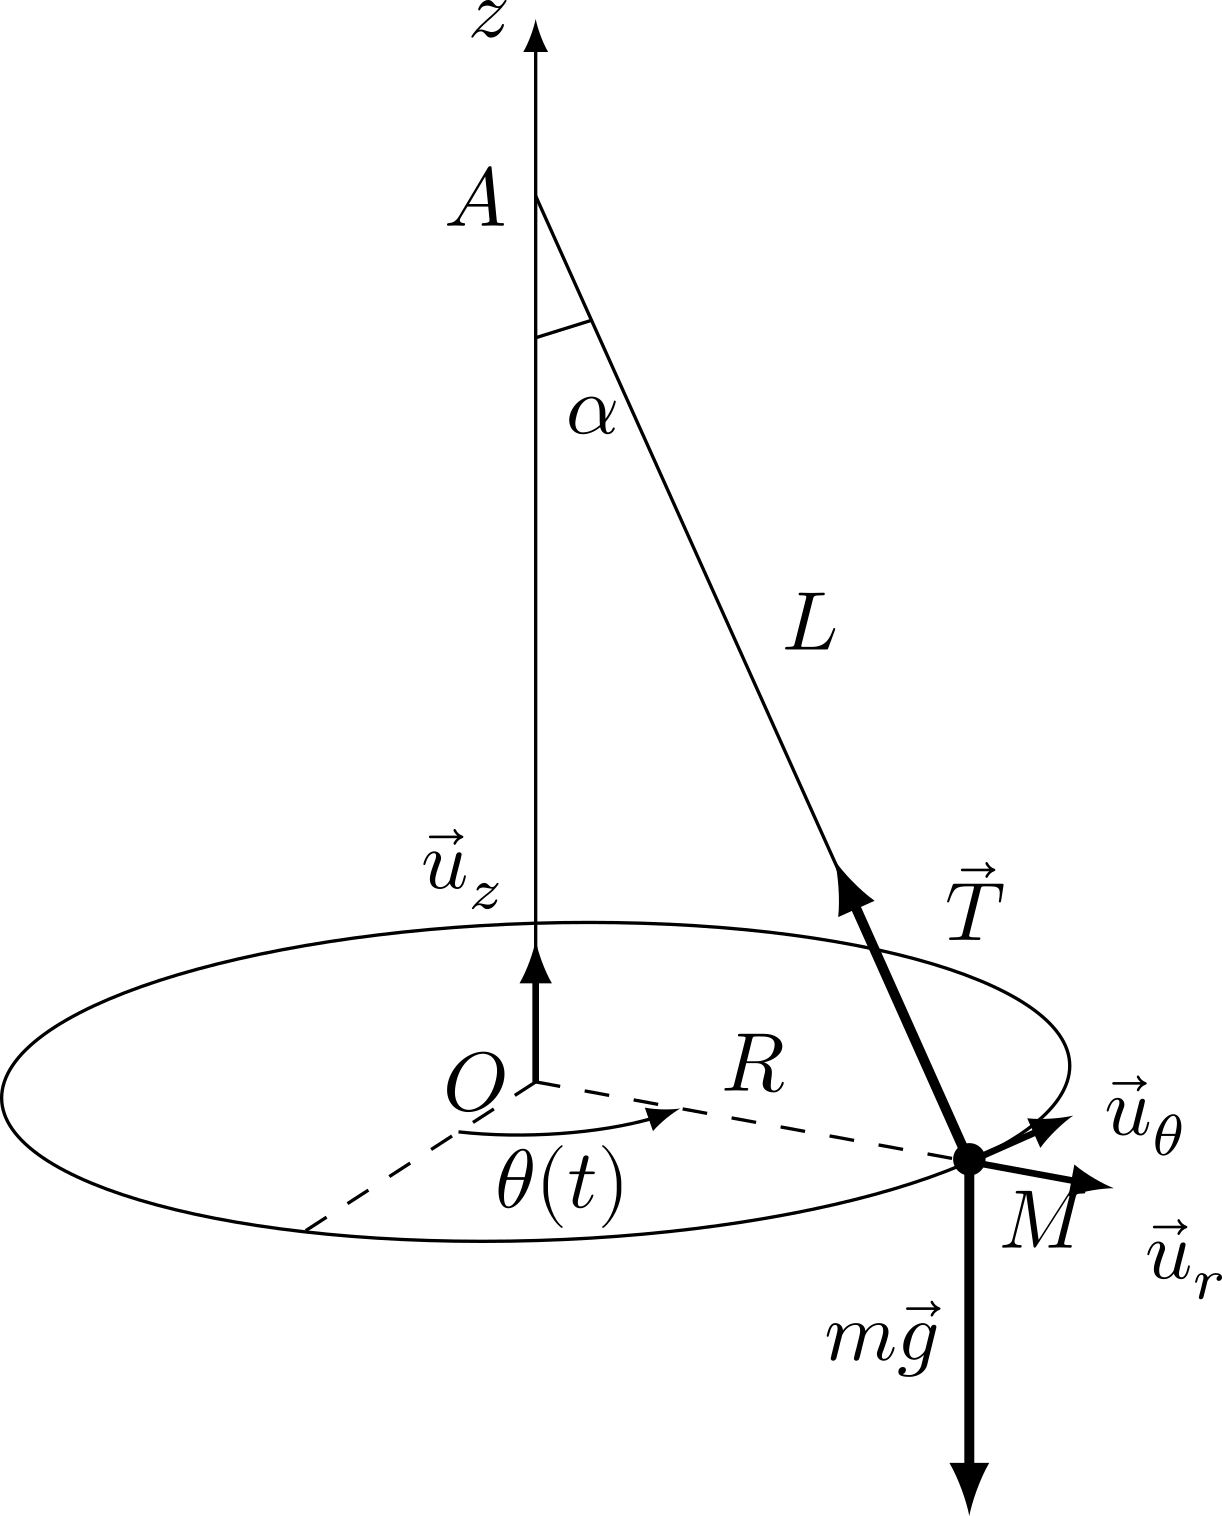
\includegraphics[width=\linewidth]{pendule_corr}
            \end{center}
        \end{minipage}
    \item On applique le PFD~:
        \begin{gather*}
            m\af = \Pf + \Tf
            \Lra
            \left\{
                \begin{aligned}
                    -mL\w^2\cancel{\sin\a} & = -T\cancel{\sin\a}\\
                    0             & = T\cos\a -mg
                \end{aligned}
            \right.
            \Lra
            \left\{
                \begin{aligned}
                    T &= mL\w^2\\
                    T &= \frac{mg}{\cos\a}
                \end{aligned}
            \right.
            \shortintertext{Soit}
            mL\w^2 = \frac{mg}{\cos\a}
            \Lra
            \boxed{\cos\a = \frac{g}{L\w^2}}
        \end{gather*}
        Pour que ce mouvement soit possible, il faut que $\cos\a < 1$, soit
        \begin{gather*}
            \frac{g}{L\w^2} < 1
            \Lra
            \boxed{\w \geq \sqrt{\frac{g}{L}} = \w_{\lim}}
        \end{gather*}
    \item Si $\w \gg \w_{\lim}$, alors $\cos\a \xrightarrow[\w \gg \w_{\lim}]{} 0$
        donc \fbox{$\a\xrightarrow[\w \gg \w_{\lim}]{} \pi/2$}~: le mouvement
        devient simplement circulaire, et se fait dans le plan horizontal
        contenant A.
    \item \leftcenters{On trouve}{\fbox{$\cos\a = \num{0.138} \Lra \a =
        \ang{82}$}}
\end{enumerate}

\end{document}
